%==================== REFERENCES ====================
\begin{thebibliography}{99}
\addcontentsline{toc}{chapter}{References}
\setlength{\itemsep}{0pt}\raggedright\urlstyle{same}

\bibitem{autogen} Q. Wu \textit{et al.}, ``AutoGen: Enabling Next-Gen LLM Applications via Multi-Agent Conversation,'' \textit{Conference on Language Modeling (COLM)}, 2024.

\bibitem{guo} T. Guo \textit{et al.}, ``Large Language Model Based Multi-agents: A Survey of Progress and Challenges,'' \textit{Proceedings of the Thirty-Third International Joint Conference on Artificial Intelligence (IJCAI)}, pp. 8048--8057, 2024.

\bibitem{react} S. Yao \textit{et al.}, ``ReAct: Synergizing Reasoning and Acting in Language Models,'' \textit{International Conference on Learning Representations (ICLR)}, 2023.

\bibitem{gan} C. Gan, Q. Zhang, and T. Mori, ``Application of LLM Agents in Recruitment: A Novel Framework for Automated Resume Screening,'' \textit{Journal of Information Processing}, vol. 32, pp. 881--893, 2024.

\bibitem{wilson} K. Wilson and A. Caliskan, ``Gender, Race, and Intersectional Bias in Resume Screening via Language Model Retrieval,'' \textit{Proceedings of the AAAI/ACM Conference on AI, Ethics, and Society (AIES)}, 2024.

\bibitem{mu} H. Mu \textit{et al.}, ``AI Security Beyond Core Domains: Resume Screening as a Case Study of Adversarial Vulnerabilities in Specialized LLM Applications,'' \textit{arXiv preprint arXiv:2512.20164}, 2025.

\bibitem{stuart} H. Stuart, M. Kaneko, and T. Baldwin, ``Beyond the Resum\'e: A Rubric-Aware Automatic Interview System for Information Elicitation,'' \textit{arXiv preprint arXiv:2603.01775}, 2026.

\bibitem{marketingfm} H. Liu, A. Tahmasbi, E. S. Haque, and P. Jain, ``LLMs for Customized Marketing Content Generation and Evaluation at Scale,'' \textit{arXiv preprint arXiv:2506.17863}, 2025.

\bibitem{selfrag} A. Asai, Z. Wu, Y. Wang, A. Sil, and H. Hajishirzi, ``Self-RAG: Learning to Retrieve, Generate, and Critique through Self-Reflection,'' \textit{International Conference on Learning Representations (ICLR)}, 2024.

\bibitem{cove} S. Dhuliawala \textit{et al.}, ``Chain-of-Verification Reduces Hallucination in Large Language Models,'' \textit{Findings of the Association for Computational Linguistics: ACL 2024}, pp. 3563--3578, 2024.

\bibitem{toolformer} T. Schick \textit{et al.}, ``Toolformer: Language Models Can Teach Themselves to Use Tools,'' \textit{Advances in Neural Information Processing Systems (NeurIPS)}, vol. 36, pp. 68539--68551, 2023.

\bibitem{gorilla} S. G. Patil, T. Zhang, X. Wang, and J. E. Gonzalez, ``Gorilla: Large Language Model Connected with Massive APIs,'' \textit{Advances in Neural Information Processing Systems (NeurIPS)}, vol. 37, 2024.

\bibitem{lukas} N. Lukas, A. Salem, R. Sim, S. Tople, L. Wutschitz, and S. Zanella-B\'eguelin, ``Analyzing Leakage of Personally Identifiable Information in Language Models,'' \textit{IEEE Symposium on Security and Privacy (SP)}, 2023.

\bibitem{mokander} J. M\"okander, J. Schuett, H. R. Kirk, and L. Floridi, ``Auditing Large Language Models: A Three-Layered Approach,'' \textit{AI and Ethics}, vol. 4, no. 4, pp. 1085--1115, 2024.

\end{thebibliography}

%==================== ACKNOWLEDGEMENT ====================
\clearpage
\addcontentsline{toc}{chapter}{Acknowledgement}
\begin{center}{\LARGE\bfseries Acknowledgement\par}\end{center}
\vspace{-5pt}
\noindent Success of a project like this, involving technical expertise, patience and the support of our guides, is possible because of the team's collaboration. We express our sincere gratitude to our internal guides, \textbf{\InternalGuideOne} and \textbf{\InternalGuideTwo}, for their continuous guidance and support throughout the project. We also extend our heartfelt thanks to our external mentor, \textbf{\ExternalMentor} (Founder \& CEO, InfinityPool Finnotech Pvt.\ Ltd.), for providing the problem statement, learning material and regular feedback through the internship reviews. Finally, we thank our college, \textbf{Fr. C. Rodrigues Institute of Technology, Vashi}, for providing the opportunity and environment to learn and grow.

\vspace{25pt}
\textbf{Project Group Members:}\par\vspace{18pt}
\MemberSignatureBlock


% =========================================================
% APPENDIX A: CODE SAMPLES
% =========================================================

%==================== APPENDIX A: CODE SAMPLES ====================
\clearpage
\phantomsection
\addcontentsline{toc}{chapter}{Appendix A: Code Samples}
\begin{center}
  {\LARGE\bfseries Appendix A: Code Samples\par}
\end{center}
\vspace{18pt}
\setcounter{lstlisting}{0}
\renewcommand{\thelstlisting}{A.\arabic{lstlisting}}

\noindent The following excerpts illustrate the core rubric-generation,
resume-screening, persistence and approval-routing logic used by the system.

\phantomsection
\noindent\textbf{A.1 Rubric Generation from Job Description}\par\vspace{8pt}
\begin{lstlisting}[language=TypeScript, caption={Generating and validating a structured rubric}]
export async function generateJDRubric(
  jobDescription: string
): Promise<JDRubric> {
  const trimmed = jobDescription?.trim();
  if (!trimmed || trimmed.length < 10) {
    throw new Error("Job description must be at least 10 characters long.");
  }

  try {
    const prompt = `
      Analyze the job description and return a JSON rubric containing:
      role_title, category, experience_years_required,
      must_have_skills, nice_to_have_skills, resume_rubric,
      and interview_rubric. Each rubric has 3-5 criteria whose
      integer weights sum to 100, with observable key indicators.

      JOB DESCRIPTION:
      ---
      ${trimmed}
      ---
    `;

    const generated = await generateStructuredJSON<JDRubric>(
      "You are an expert talent acquisition specialist. Return a structured rubric as JSON.",
      prompt,
      { temperature: 0.0 }
    );

    const validation = JDRubricSchema.safeParse(generated);
    if (validation.success) {
      const rubric = validation.data;
      rubric.resume_rubric = normalizeRubricWeights(rubric.resume_rubric);
      rubric.interview_rubric = normalizeRubricWeights(rubric.interview_rubric);
      return rubric;
    }
  } catch (error) {
    console.warn("Rubric generation failed; using the deterministic fallback.", error);
  }

  return generateMockJDRubric(trimmed);
}
\end{lstlisting}

\phantomsection
\noindent\textbf{A.2 Resume Screening and Score Storage}\par\vspace{8pt}
\begin{lstlisting}[language=TypeScript, caption={Scoring a resume and persisting its result}]
const result = await generateStructuredJSON<Record<string, unknown>>(
  SYSTEM_SCREENING_PROMPT,
  buildCandidateScreeningPrompt(job, candidate, rubric, candidateName, expYears),
  { temperature: 0.1 }
);

const rubricScores =
  result.rubric_scores && typeof result.rubric_scores === "object"
    ? result.rubric_scores as Record<string, number>
    : {};

const score = calculateHybridScore(rubricScores, rubric);

const { data, error } = await supabase
  .from("applications")
  .update({
    resume_rank_score: score,
    resume_breakdown_json: { rubric_scores: rubricScores },
    recruiter_notes: String(result.overall_summary ?? ""),
  })
  .eq("job_id", jobId)
  .eq("candidate_id", candidateId)
  .neq("status", "rejected")
  .is("deleted_at", null)
  .select("id");

if (error) {
  throw new Error(`Could not save screening result: ${error.message}`);
}
if (!data?.length) {
  throw new Error("No eligible application was found to update.");
}

const { error: statusError } = await supabase
  .from("applications")
  .update({ status: "in_progress" })
  .eq("id", data[0].id)
  .eq("current_round", "Resume Screening");

if (statusError) {
  throw new Error(`Could not update application status: ${statusError.message}`);
}
\end{lstlisting}

\phantomsection
\noindent\textbf{A.3 Workflow Router and Approval Gate}\par\vspace{8pt}
\begin{lstlisting}[language=TypeScript, caption={Routing HR decisions and gating interview approval}]
const body = await req.json();
const { jobId, decision, notes } = body;

if (!jobId || !["approved", "rejected", "pending"].includes(decision)) {
  return NextResponse.json({ success: false, error: "Invalid decision." }, { status: 400 });
}

const company = await getCurrentHrCompany();
if (!company) {
  return NextResponse.json({ success: false, error: "HR access required." }, { status: 403 });
}
if (!await ownsCompanyApplication(company.companyId, jobId, candidateId)) {
  return NextResponse.json({ success: false, error: "Application not found." }, { status: 404 });
}

if (decision === "approved") {
  const approval = await approveApplicationAndNotify({ jobId, candidateId, notes });
  if (!approval.transitioned && !approval.alreadyInInterview) {
    return NextResponse.json(
      { success: false, error: approval.failureReason },
      { status: 409 }
    );
  }
} else {
  await updateApplicationDecision(jobId, candidateId, decision, notes);
}

// Automatic approval is requested only after a successful screening score
// exceeds the job's configured threshold.
if (
  !evaluation.ai_failed &&
  Number.isFinite(evaluation.internal_score) &&
  evaluation.internal_score > job.auto_approve_threshold
) {
  await approveApplicationAndNotify({
    jobId,
    candidateId: evaluation.candidate_id,
    automatic: true,
  });
}

// The approval service claims the transition transactionally before sending
// the invitation. Automatic approvals require an open job and eligible round.
const claim = await claimApplicationForInterview({
  jobId,
  candidateId,
  notes,
  automatic,
});

if (claim.kind === "transitioned") {
  await sendCandidateApprovalEmail({ jobId, candidateId });
}
\end{lstlisting}


% =========================================================
% APPENDIX B: PLAGIARISM REPORT
% =========================================================

\clearpage
\phantomsection
\addcontentsline{toc}{chapter}{Appendix B: Plagiarism Report}
\begin{center}
    {\LARGE\bfseries Appendix B: Plagiarism Report\par}
\end{center}
\vspace*{-6pt}
\begin{center}
  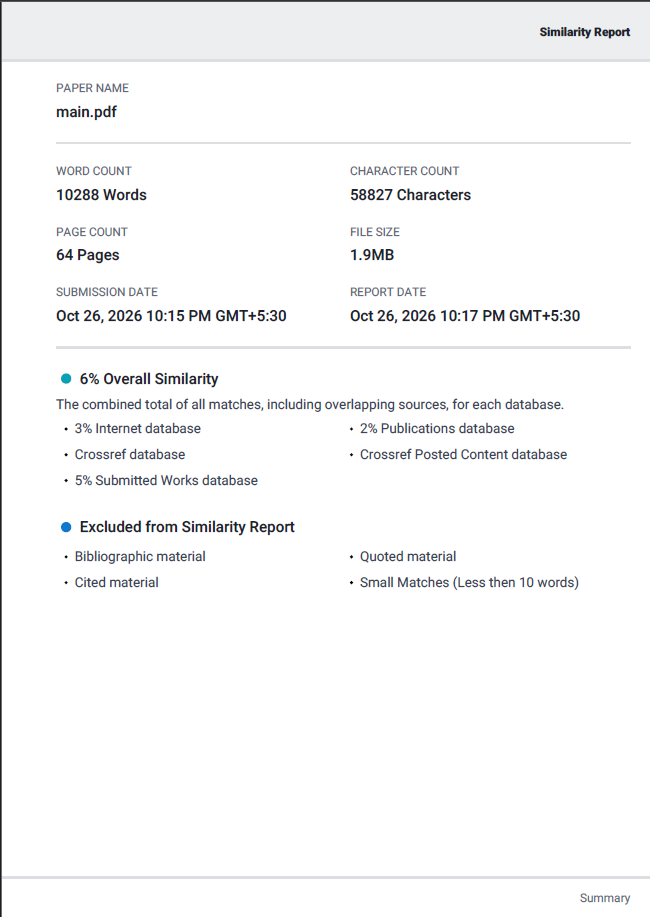
\includegraphics[width=\textwidth,height=0.85\textheight,keepaspectratio]{images/Plagarism_report.png}
\end{center}
\clearpage

% =========================================================
% APPENDIX C: T-52 PROJECT INFORMATION
% =========================================================

%==================== APPENDIX C: T-52 PROJECT INFORMATION ====================
\clearpage
\phantomsection
\addcontentsline{toc}{chapter}{Appendix C: T-52 Project Information}
\thispagestyle{plain}
\begingroup
\small

\begin{center}
  \textit{Agnel Charities}\par
  
\includegraphics[width=1.5cm]{images/fcrit_logo}\par
  \textbf{Fr. C. Rodrigues Institute of Technology, Vashi}\par
  (An Autonomous Institute and Permanently Affiliated to University of Mumbai)\par
  \vspace{5pt}
  \hfill\textit{T-52}\par
  \vspace{24pt}
  \textbf{Department of Information Technology}\par
  \textbf{Mini / Major Project Report Appendix C}
\end{center}

\vspace{8pt}
\renewcommand{\arraystretch}{1.12}
\noindent\begin{tabular}{|p{0.31\textwidth}|p{0.62\textwidth}|}
\hline
\textbf{Semester \& Academic Year:} & Semester VII, Academic Year 2026--27\\
\hline
\textbf{Group Details:} &
\StudentOne{} (\RollOne), \StudentTwo{} (\RollTwo),\newline
\StudentThree{} (\RollThree), \StudentFour{} (\RollFour)\\
\hline
\textbf{Title:} & \FullTitle\\
\hline
\textbf{Key Domain / Technology:} &
Agentic AI and multi-agent LLM workflows; Next.js, React, TypeScript,
Supabase, retrieval-augmented generation, rubric-based screening,
human-in-the-loop approvals, and audit logging.\\
\hline
\textbf{Category-I:} &
External -- \Partner\ (InfinityPool Finnotech Pvt Ltd).\\
\hline
\textbf{Category-II:} &
Application / Product -- a prototype platform for supervised business
workflows across HR, marketing, podcast research, and enterprise integrations.\\
\hline
\textbf{SDG:} & SDG 1, SDG 2, SDG 4\\
\hline
\textbf{Mapping to POs:} &
PO1, PO2, PO3, PO4, PO5, PO6, PO7, PO8, PO9, PO10, PO11\\
\hline
\textbf{Mapping to PSOs:} & PSO1, PSO2, PSO3\\
\hline
\textbf{Remarks:} & \rule{0pt}{1.3cm}\\
\hline
\end{tabular}

\vspace{10pt}
\noindent\textbf{Name and Signature of the Guide}

\vspace{16pt}
\noindent
\begin{tabular*}{\textwidth}{@{\extracolsep{\fill}}p{0.46\textwidth}}
  \rule{5cm}{0.1pt}\\[6pt]
  \IndustryGuide
\end{tabular*}

\vspace{12pt}
\noindent\textit{Note: The guide should write remarks based on the
observation of the project's objectives, achievements, and outcomes.}
\par
\endgroup


% =========================================================
% APPENDIX D: INTERNSHIP COMMENCEMENT LETTERS
% =========================================================

\clearpage
\phantomsection
\addcontentsline{toc}{chapter}{Appendix D: Internship Commencement Letters}
\begin{center}
    {\LARGE\bfseries Appendix D: Internship Commencement Letters\par}
\end{center}
\vspace{10pt}
%==================== APPENDIX D: INTERNSHIP COMMENCEMENT LETTERS ====================
\newcommand{\InternshipLetter}[1]{%
  \small
  \noindent
  \begin{minipage}[c]{0.18\textwidth}
    
\includegraphics[width=2.1cm]{images/internship_letter_logo.png}
  \end{minipage}
  \hfill
  \begin{minipage}[c]{0.78\textwidth}
    \centering
    {\Large\bfseries InfinityPool Finnotech Private Limited\par}
    CIN U74999PN2022PTC213334\par
    Reg. Address: 603, Solitaire Five, Bibwewadi, Pune-37, MH, India\par
    Corp. Address: World Trade Center, Tower 5, Kharadi, Pune-14, MH, India\par
    Web: InfinityPool.in \quad Phone: +91 980 1008 108
  \end{minipage}
  \par\vspace{10pt}\hrule\vspace{14pt}
  \begin{flushright}Date: 16 June 2026\end{flushright}
  \noindent\textbf{INTERNSHIP COMMENCEMENT LETTER}\par\vspace{18pt}
  \noindent To,\par
  #1,\par
  FCRIT, Vashi, Navi Mumbai\par\vspace{8pt}
  \noindent Dear #1,\par\vspace{6pt}
  \noindent In accordance with the Memorandum of Understanding (MoU)
  between InfinityPool Finnotech Pvt Ltd (IFPL) and Agnel Charities'
  Fr. Conceicao Rodrigues Institute of Technology (FCRIT), we would like
  to extend our heartiest congratulations on your selection as
  ``Software Engineering Intern'' with IFPL. Your internship shall
  commence on June 16, 2026 and shall end on May 30, 2027 (the ``Term'').
  You will be required to report to Mr. Mahadev Walekar during this
  internship. Our team at IFPL looks forward to having you work with us.
  \par\vspace{6pt}
  \noindent During your internship, you will be working on applying
  Artificial Intelligence techniques to solve problems in the Finance
  domain. Complete details of the project have been separately shared
  with you by IFPL. Your participation and contributions to the project
  will be subject to the terms and conditions of the non-disclosure
  agreement signed by you with IFPL. Any breach found in this regard will
  result in permissible action and immediate termination of the project.
  You may work from home during this Term. On successful completion of
  the internship, your supervisor may recommend you for a full-time offer
  of employment.
  \par\vspace{6pt}
  \noindent Once again, congratulations on your selection, and all the
  best for your endeavors.
  \par\vspace{6pt}
  \noindent Sincerely,\par\vspace{2pt}
  
\includegraphics[width=1.6cm]{images/internship_letter_signature.jpeg}\par
  Akshay Kunkulol\par
  Founder \& CEO\par\vfill
  \hrule\vspace{5pt}
  \small For verification of this document, please email
  contact@infinitypool.in\normalsize
  \clearpage
  \large
}

\InternshipLetter{Krish Pinto}
\InternshipLetter{Jerin Reji}
\InternshipLetter{Samuel Rodrigues}
\InternshipLetter{Ved Teredesai}
\renewcommand{\InternshipLetter}[1]{}


% =========================================================
% APPENDIX E: TIMELINE CHART
% =========================================================

\clearpage
\phantomsection
\addcontentsline{toc}{chapter}{Appendix E: Timeline Chart}
\begin{center}
    {\LARGE\bfseries Appendix E: Timeline Chart\par}
\end{center}
\vspace{8pt}

\begin{figure}[!htbp]
    \centering
    % Appendix E - Semester 7 Gantt Chart with Milestones
% Requires: \usepackage{pgfgantt}

\begin{ganttchart}[
    time slot format=isodate,
    x unit=0.052cm,
    y unit chart=0.80cm,
    hgrid,
    vgrid={*{6}{draw=gray!20}},
    title/.style={draw=none, fill=blue!12},
    title label font=\small\bfseries,
    bar/.style={fill=blue!50, draw=blue!75!black, rounded corners=2pt},
    bar height=0.52,
    bar label font=\footnotesize,
    bar label node/.append style={text width=5.5cm, align=right},
    group/.style={fill=blue!75!black},
    group label font=\small\bfseries,
    milestone/.style={fill=orange!90!black, draw=orange!60!black,
                      shape=diamond, inner sep=2pt},
    milestone height=0.55,
    milestone label font=\footnotesize\bfseries,
    milestone label node/.append style={text width=5.5cm, align=right},
    today=2026-10-26,
    today label=Today,
    today label font=\tiny\color{red!70!black},
    today rule/.style={draw=red!65!black, dashed, line width=0.8pt},
    canvas/.style={draw=gray!35}
]{2026-07-11}{2026-12-31}

\gantttitlecalendar{year, month=shortname} \\

\ganttbar{Environment, Python \& GitHub setup}{2026-07-11}{2026-07-24} \\
\ganttbar{AI coding tools}{2026-07-25}{2026-07-31} \\
\ganttmilestone{M1: Dev environment ready}{2026-07-31} \\
\ganttbar{LLM foundations}{2026-08-01}{2026-08-14} \\
\ganttbar{Agentic workflow foundations}{2026-08-15}{2026-08-28} \\
\ganttmilestone{M2: Agent framework POC}{2026-08-28} \\
\ganttbar{RAG, vector stores \& memory}{2026-08-29}{2026-09-11} \\
\ganttbar{n8n \& webhook automation}{2026-09-12}{2026-09-25} \\
\ganttmilestone{M3: RAG pipeline working}{2026-09-25} \\
\ganttbar{Deployment, logging \& secrets}{2026-09-26}{2026-10-09} \\
\ganttbar{Delivery kickoff \& use-case mapping}{2026-10-10}{2026-10-23} \\
\ganttmilestone{M4: Review 1 -- learning phase complete}{2026-10-23} \\
\ganttbar{HR Workflow Expansion v1}{2026-10-24}{2026-11-06} \\
\ganttbar{HR Follow-up \& Evaluation Agent}{2026-11-07}{2026-11-20} \\
\ganttmilestone{M5: Review 2 -- HR workflow demo}{2026-11-20} \\
\ganttbar{Marketing Workflow Expansion v1}{2026-11-21}{2026-12-04} \\
\ganttbar{Marketing Analytics \& Repurposing Agent}{2026-12-05}{2026-12-18} \\
\ganttmilestone{M6: Review 3 -- Marketing workflow demo}{2026-12-18} \\
\ganttbar{Podcast Guest Background Report Agent v1}{2026-12-19}{2026-12-31}

\end{ganttchart}

    \caption{\textbf{Timeline Chart of the Project
    Development -- Semester 7 (July--December 2026)}}
    \label{fig:timeline-sem7}
\end{figure}

\clearpage

\begin{figure}[!htbp]
    \centering
    % Appendix E - Semester 8 Gantt Chart with Milestones
% Requires: \usepackage{pgfgantt}

\begin{ganttchart}[
    time slot format=isodate,
    x unit=0.063cm,
    y unit chart=0.92cm,
    hgrid,
    vgrid={*{4}{draw=gray!20}},
    title/.style={draw=none, fill=teal!12},
    title label font=\small\bfseries,
    bar/.style={fill=teal!45, draw=teal!70!black, rounded corners=2pt},
    bar height=0.52,
    bar label font=\footnotesize,
    bar label node/.append style={text width=5.5cm, align=right},
    group/.style={fill=teal!75!black},
    group label font=\small\bfseries,
    milestone/.style={fill=orange!90!black, draw=orange!60!black,
                      shape=diamond, inner sep=2pt},
    milestone height=0.55,
    milestone label font=\footnotesize\bfseries,
    milestone label node/.append style={text width=5.5cm, align=right},
    canvas/.style={draw=gray!35}
]{2027-01-01}{2027-04-30}

\gantttitlecalendar{year, month=shortname} \\

\ganttbar{Sensitive research guardrails}{2027-01-02}{2027-01-15} \\
\ganttbar{Zoho Integration POC}{2027-01-16}{2027-01-29} \\
\ganttmilestone{M7: Review 4 -- Podcast \& Zoho demo}{2027-01-29} \\
\ganttbar{Workday / Greenhouse / generic HRMS POC}{2027-01-30}{2027-02-12} \\
\ganttbar{Human-in-the-loop approval flow}{2027-02-13}{2027-02-26} \\
\ganttmilestone{M8: Review 5 -- Integration demo}{2027-02-26} \\
\ganttbar{Reusable business workflow framework}{2027-02-27}{2027-03-12} \\
\ganttbar{Security, privacy \& audit logs}{2027-03-13}{2027-03-26} \\
\ganttmilestone{M9: Review 6 -- Governance \& hardening}{2027-03-26} \\
\ganttbar{Integrated demo dry run}{2027-03-27}{2027-04-09} \\
\ganttmilestone{M10: Full integrated demo approved}{2027-04-09} \\
\ganttbar{Final improvements}{2027-04-10}{2027-04-23} \\
\ganttbar{Final presentation \& handover}{2027-04-24}{2027-04-30} \\
\ganttmilestone{M11: Project complete \& submitted}{2027-04-30}

\end{ganttchart}

    \caption{\textbf{Timeline Chart of the Project
    Development -- Semester 8 (January--April 2027)}}
    \label{fig:timeline-sem8}
\end{figure}

% =========================================================
% APPENDIX F: SOFTWARE REQUIREMENTS SPECIFICATION (SRS)
% =========================================================

%==================== APPENDIX F: SOFTWARE REQUIREMENTS SPECIFICATION ====================
\clearpage
\phantomsection
\addcontentsline{toc}{chapter}{Appendix F: Software Requirements Specification}
\begin{center}
  {\LARGE\bfseries Appendix F: Software Requirements Specification\par}
\end{center}
\vspace{18pt}

%------------------------------------------------------------------
\section*{1. Introduction}

\noindent\textbf{1.1 Purpose}\\
This Software Requirements Specification (SRS) defines the functional and non-functional requirements for \textbf{\ProjectTitle{}}, an integrated multi-agent AI platform for HR recruitment, marketing content operations, podcast guest research and enterprise integrations. The document is intended for the development team, academic supervisors and industry partners at \Partner{}.

\vspace{8pt}
\noindent\textbf{1.2 Scope}\\
\ProjectTitle{} automates repetitive business workflows across HR, marketing and podcast production using specialised LLM agents coordinated by a workflow router. The system provides rubric-based resume screening, AI-conducted interviews, channel-specific content drafting, source-backed guest briefings and secure connectors to Zoho, Workday-style and Greenhouse-style APIs. It does not make final hiring, rejection, salary or publishing decisions autonomously; every consequential action requires human approval.

\vspace{8pt}
\noindent\textbf{1.3 Definitions, Acronyms, and Abbreviations}

\renewcommand{\arraystretch}{1.15}
\noindent\begin{tabular}{|p{0.28\textwidth}|p{0.65\textwidth}|}
\hline
\textbf{Term} & \textbf{Definition} \\ \hline
LLM & Large Language Model \\ \hline
RAG & Retrieval-Augmented Generation \\ \hline
ATS & Applicant Tracking System \\ \hline
HRMS & Human Resource Management System \\ \hline
PII & Personally Identifiable Information \\ \hline
OAuth & Open Authorisation (industry-standard protocol for access delegation) \\ \hline
JD & Job Description \\ \hline
API & Application Programming Interface \\ \hline
HR & Human Resources \\ \hline
CRM & Customer Relationship Management \\ \hline
n8n & Node-based workflow automation platform \\ \hline
pgvector & PostgreSQL extension for vector similarity search \\ \hline
\end{tabular}

\vspace{8pt}
\noindent\textbf{1.4 References}\\
Industry partner milestone plan and problem statement provided by \Partner{}; fortnightly review presentations (July--October 2026); IEEE Std 29148-2018 Systems and Software Engineering -- Life cycle processes -- Requirements engineering.

%------------------------------------------------------------------
\vspace{16pt}
\section*{2. Overall Description}

\noindent\textbf{2.1 Product Perspective}\\
\ProjectTitle{} is a standalone web-based platform that integrates with external enterprise systems through a connector layer. The front end is a Next.js dashboard; the back end comprises a workflow router, domain-specific LLM agents, a RAG knowledge layer, a compliance reviewer, a human approval gate and an audit store backed by Supabase. The system does not replace existing HRMS or ATS products; it orchestrates work across them.

\vspace{8pt}
\noindent\textbf{2.2 Product Functions}\\
The major functions of the system are:
\begin{itemize}
  \item Rubric generation from a job description, followed by HR review and approval.
  \item Resume parsing, adversarial-content scanning, claim verification and rubric-based scoring.
  \item AI-conducted live interviews with rubric-aligned scoring and final candidate ranking.
  \item HR assistant for onboarding, leave, attendance and policy queries.
  \item Content calendar, campaign brief and channel-specific draft generation for marketing teams.
  \item Podcast guest background reports with every claim labelled as a fact, allegation or opinion.
  \item Enterprise data synchronisation with Zoho People, Zoho CRM and Recruit, Workday-style APIs and Greenhouse-style ATS objects.
  \item Human approval queues, PII redaction, compliance review and immutable audit logging.
\end{itemize}

\vspace{8pt}
\noindent\textbf{2.3 User Characteristics}\\
\begin{itemize}
  \item \textbf{HR Recruiter:} Intermediate computer literacy; creates jobs, reviews rubrics and ranking lists, makes hiring decisions.
  \item \textbf{Candidate:} General public; submits a resume and completes an AI interview via a public link.
  \item \textbf{Marketing User:} Non-technical; creates content themes and manages the approval queue.
  \item \textbf{Podcast Host / Researcher:} Moderate technical literacy; requests and reviews guest briefings.
  \item \textbf{Administrator:} Technical; configures connectors, OAuth accounts and system settings.
\end{itemize}

\vspace{8pt}
\noindent\textbf{2.4 Constraints}
\begin{itemize}
  \item Development uses only synthetic, publicly available or sanitised data; no live client PII.
  \item Enterprise integrations use sandbox, trial or mock APIs during development.
  \item Hosted LLM costs must be minimised; local models via Ollama are used for development and testing.
  \item The system must run on the developers' existing hardware for development; production deployment targets free or low-cost hosting tiers.
\end{itemize}

\vspace{8pt}
\noindent\textbf{2.5 Assumptions and Dependencies}
\begin{itemize}
  \item Google Gemini and OpenAI API endpoints are available and responsive.
  \item Supabase PostgreSQL, Storage and pgvector are accessible with the configured credentials.
  \item Zoho, Workday-style and Greenhouse-style sandbox APIs maintain their documented schema.
  \item n8n community edition is self-hosted and reachable from the backend.
\end{itemize}

%------------------------------------------------------------------
\vspace{16pt}
\section*{3. Specific Requirements}

\noindent\textbf{3.1 External Interfaces}

\textit{User Interfaces:} A Next.js web dashboard with separate views for HR recruitment, marketing, podcast research, integrations, human review and audit log. A public candidate apply page accessible without login. Approval queue items show the full agent output, evidence and approve/edit/reject actions.

\textit{Software Interfaces:} Supabase REST and Realtime APIs for data, storage, authentication and vector search; Google Gemini and OpenAI completion and embedding endpoints; Zoho People and Recruit APIs; Workday-style HRIS API stub; Greenhouse Harvest API; Meta Marketing API; Mailchimp Marketing API; Google Calendar and Sheets APIs; n8n webhook endpoints.

\textit{Hardware Interfaces:} No direct hardware interfaces; the system is entirely web-based.

\textit{Communication Interfaces:} HTTPS for all client--server and server--API communication; OAuth 2.0 for enterprise connector authentication; webhook payloads over HTTPS for event-driven flows.

\vspace{10pt}
\noindent\textbf{3.2 Functional Requirements}

\renewcommand{\arraystretch}{1.12}
\noindent\begin{tabular}{|p{0.13\textwidth}|p{0.80\textwidth}|}
\hline
\textbf{ID} & \textbf{Requirement} \\ \hline
REQ-01 & The system shall classify every incoming request and route it to the correct HR, marketing, podcast research or integration workflow. \\ \hline
REQ-02 & The system shall generate resume and interview rubrics from a job description and present them for HR review and approval before use. \\ \hline
REQ-03 & The system shall parse uploaded resumes, scan them for adversarial content, verify material claims against public sources and score them against the approved rubric with evidence citations. \\ \hline
REQ-04 & Candidates whose resume score exceeds the HR-configured threshold shall be auto-qualified; others shall be queued for HR approval. \\ \hline
REQ-05 & The system shall conduct live AI interviews, score each answer against the interview rubric and produce a ranked shortlist with scorecards for HR review. \\ \hline
REQ-06 & The system shall answer employee queries about onboarding, leave, attendance and HR policy by retrieving from company documents and Zoho People data, citing the source. \\ \hline
REQ-07 & The system shall generate marketing content calendars, campaign briefs, audience segments and channel-specific post drafts from a provided theme or source content, guided by a stored brand knowledge base. \\ \hline
REQ-08 & All marketing drafts shall be held in an approval queue; the system shall publish only after a human approves. \\ \hline
REQ-09 & The system shall produce podcast guest briefings covering career timeline, expertise map, prior interviews, suggested questions and sensitive topics, with every claim attributed to a cited source and labelled as a verified fact, allegation or opinion. \\ \hline
REQ-10 & The system shall read and write data in Zoho, Workday-style and Greenhouse-style systems through a typed connector interface that handles OAuth, pagination, rate limits, retries and idempotency. \\ \hline
REQ-11 & All external write operations and public communications, except auto-qualified interview invitations, shall wait for explicit human approval recorded in the audit log. \\ \hline
REQ-12 & The system shall store, for every workflow run, the prompt, tool calls, retrieved sources, draft versions, reviewer identity and final output in an immutable audit log. \\ \hline
\end{tabular}

\vspace{10pt}
\noindent\textbf{3.3 Usability Requirements}
\begin{itemize}
  \item HR and marketing staff with no AI background shall be able to use the dashboard and approval queues without training beyond a brief orientation.
  \item Approval queue items must display the full agent rationale and evidence so that a reviewer can make an informed decision without consulting other systems.
  \item The candidate apply page and interview interface must be accessible to applicants on standard desktop and mobile browsers without any account creation.
\end{itemize}

\vspace{10pt}
\noindent\textbf{3.4 Performance Requirements}
\begin{itemize}
  \item Resume screening results shall be produced within 60 seconds of submission for a standard two-page resume.
  \item AI interview responses shall be generated within 5 seconds of each candidate answer to maintain a conversational pace.
  \item Marketing draft generation for a five-post calendar shall complete within 90 seconds.
  \item Connector sync operations shall complete within 30 seconds for standard paginated fetches of up to 100 records.
\end{itemize}

\vspace{10pt}
\noindent\textbf{3.5 Logical Data Requirements}\\
Jobs, rubrics, candidates, applications, scores, interview transcripts, marketing campaigns, post drafts, guest briefings, connector accounts and audit events are stored in Supabase PostgreSQL. Resume files and multimedia attachments are stored in Supabase private storage buckets. Embeddings for the knowledge base are indexed using pgvector. Retention of candidate PII is limited to the duration of the hiring process; deletion requests are honoured within the same working day.

\vspace{10pt}
\noindent\textbf{3.6 Security and Safety Requirements}
\begin{itemize}
  \item API keys, OAuth tokens and database credentials must be stored in environment variables and must never appear in source code, prompts or logs.
  \item Candidate PII must be redacted from LLM prompts before scoring; only anonymised content is sent to external model APIs.
  \item Resume files must be stored in private buckets accessible only through signed, time-limited URLs.
  \item All connector write operations require an HR-approved scope; least-privilege OAuth scopes must be used.
  \item Resumes must be scanned for hidden instructions before scoring; flagged files must be routed to a human review queue.
  \item Role-based access control must prevent candidates from accessing recruiter views and prevent marketing users from accessing HR data.
\end{itemize}

\vspace{10pt}
\noindent\textbf{3.7 Quality Attributes / Non-Functional Requirements}
\begin{itemize}
  \item \textbf{Reliability:} Connector calls must implement exponential back-off retries and idempotency keys so that transient failures and duplicate events do not create duplicate records.
  \item \textbf{Maintainability:} New agents, connectors and business functions must be addable through the reusable workflow framework without modifying the router core.
  \item \textbf{Evaluability:} Each workflow must be exercisable against a synthetic test suite; accuracy, hallucination rate, latency and task completion rate must be measurable.
  \item \textbf{Portability:} The backend must be deployable on any Node.js-compatible hosting platform; connector configuration must be isolated in environment variables.
  \item \textbf{Auditability:} Every output must be traceable from the final decision back to the initiating prompt, tool calls, retrieved sources and reviewer within the audit log.
\end{itemize}

%------------------------------------------------------------------
\vspace{16pt}
\section*{4. Verification / Acceptance Criteria}

\renewcommand{\arraystretch}{1.12}
\noindent\begin{tabular}{|p{0.13\textwidth}|p{0.25\textwidth}|p{0.54\textwidth}|}
\hline
\textbf{Req. ID} & \textbf{Method} & \textbf{Criterion} \\ \hline
REQ-01 & Test execution & Given ten sample requests across all four domains, the router correctly classifies all ten. \\ \hline
REQ-02 & Demonstration & HR user uploads a JD and receives a structured rubric within 30 seconds; rubric is editable and saveable. \\ \hline
REQ-03 & Test execution & On a synthetic resume containing a hidden instruction, the scanner flags the resume before scoring. \\ \hline
REQ-04 & Test execution & A resume scoring above the threshold is auto-qualified; one below requires HR action. \\ \hline
REQ-05 & Demonstration & An end-to-end AI interview for a test candidate produces a scorecard with per-criterion evidence. \\ \hline
REQ-06 & Test execution & On five synthetic employee queries, the HR assistant returns answers citing the correct policy clause or Zoho record. \\ \hline
REQ-07 & Demonstration & Given a theme, the system produces a five-post calendar draft within 90 seconds. \\ \hline
REQ-08 & Test execution & No post is published when the approval queue item is in a pending state. \\ \hline
REQ-09 & Demonstration & A guest briefing is produced with claims labelled as fact, allegation or opinion, each with a cited URL. \\ \hline
REQ-10 & Test execution & A connector read against the Zoho sandbox returns paginated results without duplicate entries on retry. \\ \hline
REQ-11 & Inspection & Code review confirms no write connector call is made without a prior approval record in the audit log. \\ \hline
REQ-12 & Inspection & Audit log entries for a sample run contain prompt hash, tool calls, source URLs, reviewer ID and final output ID. \\ \hline
\end{tabular}

%------------------------------------------------------------------
\vspace{16pt}
\section*{5. Supporting Information}

\noindent\textbf{Appendix A -- Traceability Matrix}

\renewcommand{\arraystretch}{1.12}
\noindent\begin{tabular}{|p{0.22\textwidth}|p{0.70\textwidth}|}
\hline
\textbf{Stakeholder Need} & \textbf{Mapped Requirements} \\ \hline
Reduce recruiter time on resume review & REQ-02, REQ-03, REQ-04, REQ-12 \\ \hline
Fair, explainable candidate scoring & REQ-02, REQ-03, REQ-05, REQ-12 \\ \hline
Prevent adversarial resume manipulation & REQ-03, REQ-06 (security scan) \\ \hline
Maintain brand consistency in marketing & REQ-07, REQ-08 \\ \hline
Fact-safe podcast guest briefings & REQ-09 \\ \hline
Secure enterprise data exchange & REQ-10, REQ-11, REQ-06 (security) \\ \hline
Full audit trail for every AI decision & REQ-11, REQ-12 \\ \hline
\end{tabular}

\vspace{10pt}
\noindent\textbf{Appendix B -- Change History}

\noindent\begin{tabular}{|p{0.15\textwidth}|p{0.15\textwidth}|p{0.62\textwidth}|}
\hline
\textbf{Version} & \textbf{Date} & \textbf{Change Summary} \\ \hline
1.0 & Oct 2026 & Initial SRS drafted from problem statement, milestone plan and existing-systems study. \\ \hline
\end{tabular}

